\documentclass[12pt,defaultstyle]{umassdthesis_new}

\usepackage[T1]{fontenc}

%\usepackage[latin1]{inputenc} %% I was getting errors

\usepackage[utf8]{inputenc}

\usepackage{graphicx}
\usepackage{multirow,hhline,dcolumn} % useful commands for Tables
%\usepackage[toc]{appendix}
%\usepackage[pages]{appendix}
\usepackage{mathrsfs} 
\usepackage{hyperref}
%\usepackage{cite}
\usepackage{float}
%%  user defined commands
\newcommand{\linefrac}[2]{\raisebox{.6ex}{#1}/\raisebox{-0.6ex}{#2}} 
\def\BibTeX{{\rm B\kern-.05em{\sc i\kern-.025em b}\kern-.08emT\kern-.1667em\lower.7ex\hbox{E}\kern-.125emX}}
\newcommand{\scri}{{\mathscr I}}


%%  the entries below should be self-explanatory, some of these entries may
%%  safely be excluded from the thesis, other are required.  LaTeX will
%%  print a warning message if a required entry is not included.

\title{Turbulently-Driven Detonation Initiation in Electron-Degenerate Matter with Helium}

\author{Gabriel}{Casabona}

\dept{Department of}{Physics}
\college{College of}{Engineering}
\conferraldate{August}{2019}

%%  select the degree being earned
%%  \degree{FULL NAME}{ABBREVIATION}
%%
%\degree{Undergraduate}{Undergraduate}
%\degree{Honors}{Honors}
%\degree{Master of Arts}{M.A.}
%\degree{Master of Art Education}{M.A.Ed.}
%\degree{Master of Fine Arts}{M.F.A.}
\degree{Master of Science}{M.S.}
\program{Physics}
%%  PhD disertations have a few extra details such as the program name
%%  this is to allow for the EAS and BMBMT programs
%%\degree{Doctor of  Philosophy}{Ph.D.}
%%  \phdprogram{PROGRAM NAME}{LABEL}
%%
%\phdprogram{Computer Engineering}{ECE}
%\phdprogram{Biomedical Engineering and Biotechnology}{BMEBT}


%%  advisors and readers have a professorial title, name and affiliation
%%  but NOT degrees earned (ie. do not write Dr. Smith )
%%
\advisor{Associate Professor, Department of Physics}{Robert Fisher}%
{Physics}{University of Massachusetts Dartmouth}

%%  co-advisors are allowed ....
%%  sometime the co-advisor "replaces" a reader but other times there are 
%%  also the full complement of readers. Undergraduate and Masters thesis
%%  have two readers while in the case of Ph.D. dissertations, there are
%%  three readers.  The classfile can cope with this ambiguity when 
%%  generating the signature page.
%% 
%\coadvisor{Associate Professor}{Fred A. Dagg}%
%{Physics}{University of Massachusetts Dartmouth}

\readerone{Professor}{Gaurav Khanna}%
{Physics}{University of Massachusetts Dartmouth}

\readertwo{Assistant Professor}{Scott Field}%
{Mathematics}{University of Massachusetts Dartmouth}

%\readerthree{Postdoctoral Associate}{James Guillochon}%
%{Center for Astrophysics}{Harvard University}

%%  the rest of the entries on the signature page have a
%%  professorial title and name (the affiliation will be UMASS DARTMOUTH)

\graddirector{Robert Fisher}
\deptchair{Jianyi Jay Wang}
\collegedean{Jean VanderGheynst}%%2217 line in .cls
\gradstudies{Tesfay Meressi}
%%  this is for Honors (undergraduate) theses
%%\honorsdirector{Catherine Gardner}





%%
%%  THE ABSTRACT
%%  ============
%%
%%  From the UMass Dartmouth Thesis Guide
%%  "Requirements for Theses and Dissertations" (Spring 2015) 
%%  
%%  5.1.4 Abstract
%%  --------------
%%  The thesis or dissertation must contain an abstract    a concise summary of
%%  the thesis or dissertation intended to inform a prospective reader about
%%  its content. It usually includes a brief description of the problem
%%  investigated, the procedures or methods used, the findings, and the
%%  conclusions. It may use one or a few paragraphs; however, it is very rare
%%  that an abstract should use more than two pages, and many use just one page. 
%%
\abstract[long]{%
Type Ia supernovae (SNe Ia) are believed to result from the thermonuclear explosions of carbon-oxygen white dwarfs.  While important as standardizable candles, and sources of nuclear enrichment and cosmic rays, the stellar progenitors, as well as the mechanism for detonation of SNe Ia are still unknown. In previous collaborative work, I have shown that a turbulently-driven mechanism can give rise to a detonation in carbon-oxygen electron-degenerate fuel in the distributed burning regime. We have now extended this turbulently-driven detonation mechanism to simulate the detonation of carbon in the presence of helium. Using high-resolution local three-dimensional hydrodynamic simulations with the FLASH4 code, I explore a range of parameter space motivated by leading progenitor models of SNe Ia. I show that the helium abundance greatly affects the range of conditions needed to detonate carbon in electron-degenerate matter. These local models can then be used in subgrid models of nuclear burning and detonation initiation in future global simulations of SNe Ia.

%%  the empty line before the closing brace is REQUIRED to ensure that 
%%  the formatting of the abstract page is done correctly
%%  !!DO NOT REMOVE THIS LINE!!

}%
%%  done the abstract !!

%%
%%  THE ACKNOWLEDGEMENTS
%%  ====================
%%
%%  From the UMass Dartmouth Thesis Guide
%%  "Requirements for Theses and Dissertations" (Spring 2015) 
%%  
%%  5.1.5 Acknowledgments
%%  ---------------------
%%  Short statements of acknowledgment of indebtedness (e.g., thanks to one  s
%%  thesis or dissertation advisor, to other professors, to people who have
%%  given support) may appear on a separate page right after the abstract. An
%%  acknowledgments section is required if the author has received permission to
%%  use previously copyrighted material or is obliged to acknowledge grant
%%  sources. This section is present in most theses or dissertations and is used
%%  to express a very specific professional or personal indebtedness. For
%%  example, significant instances of collaboration with one or more others in
%%  one  s thesis or dissertation work would probably need acknowledgment in a
%%  Preface (see 5.1.8) or in this Acknowledgments section  for example, research
%%  undertaken together with another student or use of much material from some
%%  other investigator.
%%
%%  The acknowledgements should be written in a professional manner. When
%%  writing the acknowledgments, be sure that your use of   person   is
%%  consistent.  If you begin with references to yourself as   the author,  
%%  continue to use third person throughout. If you begin with first person
%%  (  I,     me,     my  ), use first person consistently.  There are two accepted
%%  spellings of the word   acknowledgments   (the other is   acknowledgements  );
%%  be sure to spell this word consistently.
%%
\acknowledgements{%
	This work used the code FLASH 4.0.1, developed by the DOE NNSA-ASC OASCR Flash Center at the University of Chicago. Simulations ran in parallel on the Extreme Science and Engineering Discovery Environment (XSEDE) Stampede2 supercomputer at the University of Texas at Austin's Texas Advanced Computing Center. Plots and analysis of our runs were done with yt. Special thanks to Professor Robert Fisher, for providing the proper guidance in physics and computational techniques to make this work possible and also for providing me with a Research Assistantship. I would also like to thank the Physics department at the University of Massachusetts Dartmouth for their continued support as I advance in my academic career, as well as the university as a whole for providing me with exceptional care to all my needs as a student. 

%%  the emply line before the closing brace is REQUIRED to ensure that 
%%  the formating of the acknowledgments page is done correctly
%%  !!DO NOT REMOVE THIS LINE!!

}%
%%  done the acknowledgements !!


%%
%%  THE PREFACE (optional)
%%  ======================
%%
%%  From the UMass Dartmouth Thesis Guide
%%  "Requirements for Theses and Dissertations" (Spring 2015) 
%%  
%%  5.1.8 Preface (optional)
%%  ------------------------
%%  Most theses or dissertations will not have a Preface, which is called for
%%  only for unusual reasons, e.g., when the genesis of the work needs to be
%%  explained or when the author  s contribution to a multiple-authored work must
%%  be noted. If there is a preface, however, it would incorporate any
%%  acknowledgments instead of those appearing as a separate section.
%%  
%%  Preface sections are rarely used.  The first chapter (sometimes called
%%    Introduction  ) in the text section is the appropriate place for
%%  explanations of the context or the motivations that underlie the research,
%%  the research problem, the background of previous scholarship, notable
%%  contributions by other scholars, and so forth. Use a   Preface   section only
%%  for special purposes beyond such purposes as these; examples of such a
%%  special purpose are covered in sections 7.4 and 8.5.
%%  
%%
%%  7.4 Translations by the Author of Material Used
%%  ----------------------------------------------- 
%%  Material that you translate is still the intellectual property of the
%%  author. It must be documented fully (its original-language source cited
%%  properly and included in the bibliography). An appropriate note indicates by
%%  whom it has been translated, by you or someone else. If a thesis or
%%  dissertation will have extensive use of such material, this might be an
%%  occasion for an explanation in a Preface.  Usually, translators of published
%%  works will be indicated in the standard documentation of your notes and/or
%%  bibliography.
%% 
%%  8.5 Collaborative Work That Will Appear in a Thesis or Dissertation
%%  -------------------------------------------------------------------
%%  A thesis or dissertation must represent work done principally if not
%%  entirely by the author. When there are minor instances of research
%%  collaboration, an appropriate citation may be used. If extensive, however,
%%  the committee must approve it in detail and an explanation in a Preface
%%  section is called for (see sections 5.1.8).
%% 
%%  
%%  The preface should be written in a professional manner. When writing the
%%  acknowledgments, be sure that your use of   person   is consistent.  If you
%%  begin with references to yourself as â the author,â  continue to use third
%%  person throughout. If you begin with first person (  I,     me,     my  ), use
%%  first person consistently.  
%%
%\preface{%
%  The text of the preface goes here.
%%%  the emply line before the closing brace is REQUIRED to ensure that 
%%%  the formatting of the preface page is done correctly
%%%  !!DO NOT REMOVE THIS LINE!!
%
%}%
%%%  done the preface !!


%%
%%  THE EPIGRAPH (optional)
%%  =======================
%%
%%  Some authors include a quotation (epigraph) or illustration (frontispiece)
%%  as the last of their preliminary pages. Neither should be listed in the
%%  table of contents, although a frontispiece may be included in the list of
%%  illustrations. The source of an epigraph is indicated below the quotation
%%  but is not listed in the bibliography or references unless it is also
%%  cited in the text. A page number need not be shown, but the page is
%%  counted in the sequential page numbering.

%%  The default option is a epigraph (text).
%%  The two LaTeX commands below will produce the same output.
%%
%\epigraph{%
%    \centering{To all of the fluffy kitties \ldots} 
%%%  the emply line before the closing brace is REQUIRED to ensure that 
%%%  the formating of the preface page is done correcty
%%%  !!DO NOT REMOVE THIS LINE!!
%
%}%
%\epigraph[epigraph]{%
%    \centering{To all of the fluffy kitties \ldots}
%%%  the empty line before the closing brace is REQUIRED to ensure that 
%%%  the formating of the preface page is done correcty
%%%  !!DO NOT REMOVE THIS LINE!!
%
%}%


%%  To include an illustration, use the optional argument of 
%%  frontispiece and the image file name as the second argument
%%
%%\epigraph[frontispiece]{einstein_bike}

%%%  done the epigraph !!


%%  need these if there are no Figure or Tables
%%  otherwise evil things happen to the Table of Contents
%\emptyLoF
%\emptyLoT

%%  uncomment to aviod generating prologue pages
%\SuspendPrologue

%%  All the prologue pages are done.  The thesis proper begins after here.

%%
%%  End of LaTeX preamble
%%  =========================================================================

%\usepackage[round]{natbib}
%\usepackage{deluxetable}
%\usepackage{bibentry}
%\nobibliography*

\newcommand {\arx} {arxiv}

%%%%%%%%%%%%%%%%%%% usepackage commands %%%%%%%%%%%%%%%%%%%%%
\usepackage{grffile}
%\usepackage{deluxetable}
%\setlength{\textfloatsep}{0.5in plus 1.0pt minus 1.0pt}
%\setlength{\floatsep}{0.25in plus 1.0pt minus 1.0pt}
%\setlength{\intextsep}{0.5in plus 1.0pt minus 1.0pt}
\usepackage{amsmath}
\usepackage{amssymb}
\usepackage{color}
\usepackage{calc}

%\graphicspath{{figures/}}

%%%%%%%%%%%%%%%%%%%%%%%%%%%%%%%%%%%%%%%%

\begin{document}


%%  set the format required for the citations/references
%%  \bibliographystyle{unsrt} is preferred for UMassD theses & dissertations.
%%\bibliographystyle{unsrt}
\bibliographystyle{plainnat}


%%  The document text can be typed directly into this file or make use of
%%  the LaTeX \input{filename} command to read the contents of the file
%%  filename.tex.
%%  The later method is a good way to logically organize the material.

%%  INSERT THESIS BODY HERE


%%  if using the LaTeX \imput command 
\chapter{Introduction}

Type Ia supernovae (SNe Ia) are the thermonuclear explosions of white dwarfs (WDs). These WDs are in binary systems, accreting matter from their companion stars. One of the many unique characteristics of SNe Ia is that they have a consistent peak luminosity, which is why they are used in cosmology as standardizable candles \cite{phillips93}. Their use as standardizable candles helped in the discovery of the accelerated expansion of the universe \cite{Riess98}. SNe Ia are also prominent sources of cosmic rays and the abundance of $^{56}$Fe in the universe.

Although it is known that SNe Ia are the thermonuclear explosions of WDs, their detonation mechanism remains unknown. In our previous work \cite{Fisher}, we proposed a detonation mechanism for carbon in electron-degenerate matter due to turbulence. Using localized 3-dimensional hydrodynamics simulations, we found that carbon can indeed detonate in electron-degenerate turbulent matter in the distributed burning regime. We refer to this new mechanism as a \textit{turbulently-driven detonation mechanism}. For this project, we explore the parameters of how the detonation of helium may lead to the detonation of carbon. Inspiration comes from previous literature that determined what role the detonation of the helium surface of the WD plays in SNe Ia.  

\section{Type Ia Supernovae}

The categorization of SNe begins with hydrogen. Type II SNe are characterized by strong hydrogen absorption lines in their spectrum. SNe II result from the collapse of a massive star, with masses greater than 10 M$_{\odot}$, at the end of their lifetime. Type I SNe have no hydrogen lines in their spectra. Furthermore, SNe Ia spectra have strong silicon absorption lines. Early models predicted that SNe Ia must come from a compact object, which was confirmed by SN 2011fe \cite{Nugent_2011}. Astronomers were able to observe the region where the event took place before and after the explosion, confirming early suspicions. The only two compact objects in the universe that can explode, as far as we know, are WD and neutron stars (NS). NS are known to explode into kilonovae, so strong confidence is put into SN 2011fe originating from a WD.

Progenitors of SNe Ia involve a primary WD in a binary system. In a single-degenerate channel, the secondary is usually a star still on main sequence. Extensive work has gone into exploring single-degenerate models, however, observational evidence does not support this channel since no surviving companion main sequence star has yet been found for a normal SN Ia event.

In the double-degenerate (DD) channel, both the primary and secondary stars are WDs. The primary WD tidally disrupts the secondary WD, creating an accretion disk around the primary. Over time, this disk accretes onto the primary WD, creating a highly turbulent environment. Motivated by the DD channel, our previous work showed that the turbulent cascade caused by the accreting matter can lead to a detonation \cite{Fisher}. Those models included electron-degenerate matter consisting of a 1:1 ratio of carbon and oxygen. For this project, we take this mechanism one step further to explore how turbulence can lead to the detonation of helium, which might then detonate carbon.   

\section{Helium Detonation Models}

WD are known to have a relatively thin helium shell around them resulting from stellar evolution \cite{giammichele}. During the merger of these binary systems, the helium of the secondary WD will accrete first and mix with the helium layer of the primary WD. Motivation for this project comes from recent literature which explores various mechanisms of the detonation of this helium layer and how this leads to the detonation of the carbon core. One of these mechanisms is called the double-detonation mechanism. In one possible scenario, two individual spots in the helium layer of the primary WD detonate, sending shock waves radially inwards towards the carbon core. At the point where the shock waves meet, carbon detonation is intitiated at an off-center location. 

In a more realistic model, the helium accretion from the secondary WD continuously adds to the helium shell of the primary WD, until the primary detonates \cite{Shen}. This mechanism adds more kinetic energy since mass is being added into the system with high velocities. Known as the dynamically driven double-degenerate double-detonation, D$^6$, SNe Ia are now modeled with a much wider range of initial conditions. An outcome of the D$^6$ model is complete detonation of the primary WD, which sends the secondary WD as a hypervelocity runaway. Recent observations from \textit{Gaia} now support the existence of this new model \cite{Gaia}, further increasing the need to explore this detonation mechanism.

\section{Turbulence}

The majority of the universe exists in a fluid state, either gas or plasma. For this reason, the study of fluid dynamics is crucial for understanding phenomenon happening in the universe. In astrophysics, modeling fluids takes the form of Euler's equation,
\begin{equation*}
	\frac{\partial (\rho \textbf{v})}{\partial t} + \nabla \bullet (\rho \textbf{vv}) = -\nabla P - \rho \nabla \Phi,
\end{equation*}
where $\rho$ is the mass density, $\textbf{v}$ is the velocity vector, $P$ is the thermal pressure, $\Phi$ is the gravitational potential, and $G$ is the universal constant of gravitation \cite{euler}. In this form, the  fluid has zero viscosity and includes effects from self-gravity. This project involves modeling electron-degenerate matter at scales much higher than those needed to have viscosity play a role, so the approximation of the Euler fluid will suffice.

In the simplest of cases, fluids are modeled as a laminar flow. This means that the velocity vector lines are all smoothly varying. Realistic cases, however, need to include turbulence, in which the velocity vector lines are no longer smooth. This is caused from chaotic changes in the fluid's velocity and pressure. The onset of turbulence typically begins with some kind of fluid instability. Rayleigh-Taylor and Kelvin-Helmholtz are two of the major instabilities found in astrophysics.

An important quantity that is needed when describing turbulence is the dimensionless Reynold's number, (Re), defined as
\begin{equation*}
	{\rm Re} = \frac{\rho u L}{\mu}.
\end{equation*}
Here, $\rho$ is the density of the fluid, $u$ is the velocity of the fluid, $L$ is the linear dimension, and $\mu$ is the dynamic viscosity of the fluid. Re above 2000 means that the fluid flow becomes turbulent. Astrophysical fluids have low viscosities, resulting in them almost always being turbulent. An important quantity here is the linear dimension, meaning that the Re number is dependent on the length scales in question, a property which will be exploited later. 

One important aspect of turbulent flow is the onset of a turbulent cascade. Kolmogorov's theory of turbulence tells us that the turbulent cascade allows for the cascade of energy. When turbulence is first initiated, its eddies are at the largest length scales, which is determined by the geometry of the system. The time-scale of these eddies is determined by its turnover time, the time it takes for one eddy to make one complete loop. As time evolves, these eddies break up and form smaller ones, which then have smaller time-scales. Once this time-scale is small enough, the viscosity of the fluid then dissipates the kinetic energy of the turbulence into heat. In our previous work, we showed that when the time-scale of the eddies reduces even lower until equaling that of the nuclear burning time-scale, this is the moment of the initiation of detonation \cite{Fisher}. Another important aspect of Kolmogorov's theory is that the turbulence becomes isotropic as the time-scales are reduced, for high Re numbers. This means that regardless of the large scale eddies, which is determined by the geometry of the system, the statistics of initial range turbulence are universal.


\section{Distributed Burning Regime}

In a regime with negligible turbulence, the nuclear burning is laminar. This flame is characterized by a length, $l$, and a speed, $s_l$. The flame maintains a well-defined structure since turbulence has little effect on it. When turbulence begins to influence the structure of the flame, we then consider the dimensionless Karlovitz number, (Ka), defined as
\begin{equation*}
	{\rm Ka} = \sqrt{\frac{v_{\rm RMS}^3}{s_l^3} \frac{l}{L}},
\end{equation*}
where $L$ is the integral scale and $v_{\rm RMS}$ is the RMS velocity at the integral scale. When Ka < 1, turbulence is low enough that the structure of flame remains intact. For Ka > 1, turbulence begins to disrupt the structure of the flame. For Ka $\gg 1$, the flame is completely disrupted by the turbulence. The flame now exists in the distributed regime, where the turbulent mixing dominates electron conduction. In regions of key interest in the double-degenerate channel of SNe Ia, Ka $\simeq 10^4$, deep into the distributed burning regime, another motivator of this project.

\section{Zel'dovich Gradient Mechanism}

To better understand the significance of the distributed burning regime, it is important to note what the leading theory was in detonation mechanisms for SNe Ia. First modeled by Zel'dovich and collaborators \cite{zeldovichetal70}, the Zel'dovich gradient mechanism describes how a laminar flame may lead to a detonation. It begins with the formation of a laminar flame in a hot background, accelerating down a temperature gradient. The formation of the flame initiates a shock front ahead of it. If the temperature gradient is shallow enough, then this initially subsonic laminar flame will accelerate just behind the shock front. The shock front leading the flame front allows for the carbon in that regime to fully burn, causing a detonation. When the temperature is too steep, the shock front will accelerate much quicker than the flame front, leaving it behind. In this case, carbon is not fully burned, causing a failed detonation. Failed detonations with the Zel'dovich gradient mechanism put a lower limit on the temperatures needed to detonate carbon. Our previous work shows with turbulence taken into consideration, critical temperatures for carbon detonation are a factor of 2-3 times lower than previous studies based upon Zel'dovich. 

\chapter{Turbulently-Driven Detonation Mechanism}

\section{Carbon Detonation}

In our previous work, we determined that our turbulently-driven detonation mechanism can lead to the detonation of carbon in electron-degenerate matter. Three-dimensional hydrodynamic simulations were carried out with electron-degenerate fuel consisting of equal ratios of carbon and oxygen in a density of $10^7$ g cm$^{-3}$. Through extensive statistical tests, detonation initiation occured when the time scale of the turbulence, characterized by the eddy-turnover time on the critical length scale, becomes larger than the nuclear burning timescale, $t_{edd}/t_{burn} \simeq 10^9$.

\begin{table}[htp]
\caption[A table of carbon-oxygen runs with different resolution, RMS velocity and mean temperature..]{Results from intitial work that established a turbulently-driven detonation mechanism using only carbon and oxygen. Mass-weighted mean temperature at the time of detonation in each resolution are listed.}
  \begin{center}
      \begin{tabular}{|c|c|c|c|}
        \hline
	      Resolution & $T_{mean}$(K) \\
        \hline\hline
        $64^3$   & $1.12 \times 10^9$ \\
	$128^3$   & $1.17 \times 10^9$ \\
	$256^3$   & $1.17 \times 10^9$ \\
	$512^3$   & $1.18 \times 10^9$ \\      
        \hline
   \end{tabular}
  \end{center}
  \label{runs}
\end{table}

\begin{center}
\begin{figure}[hp]

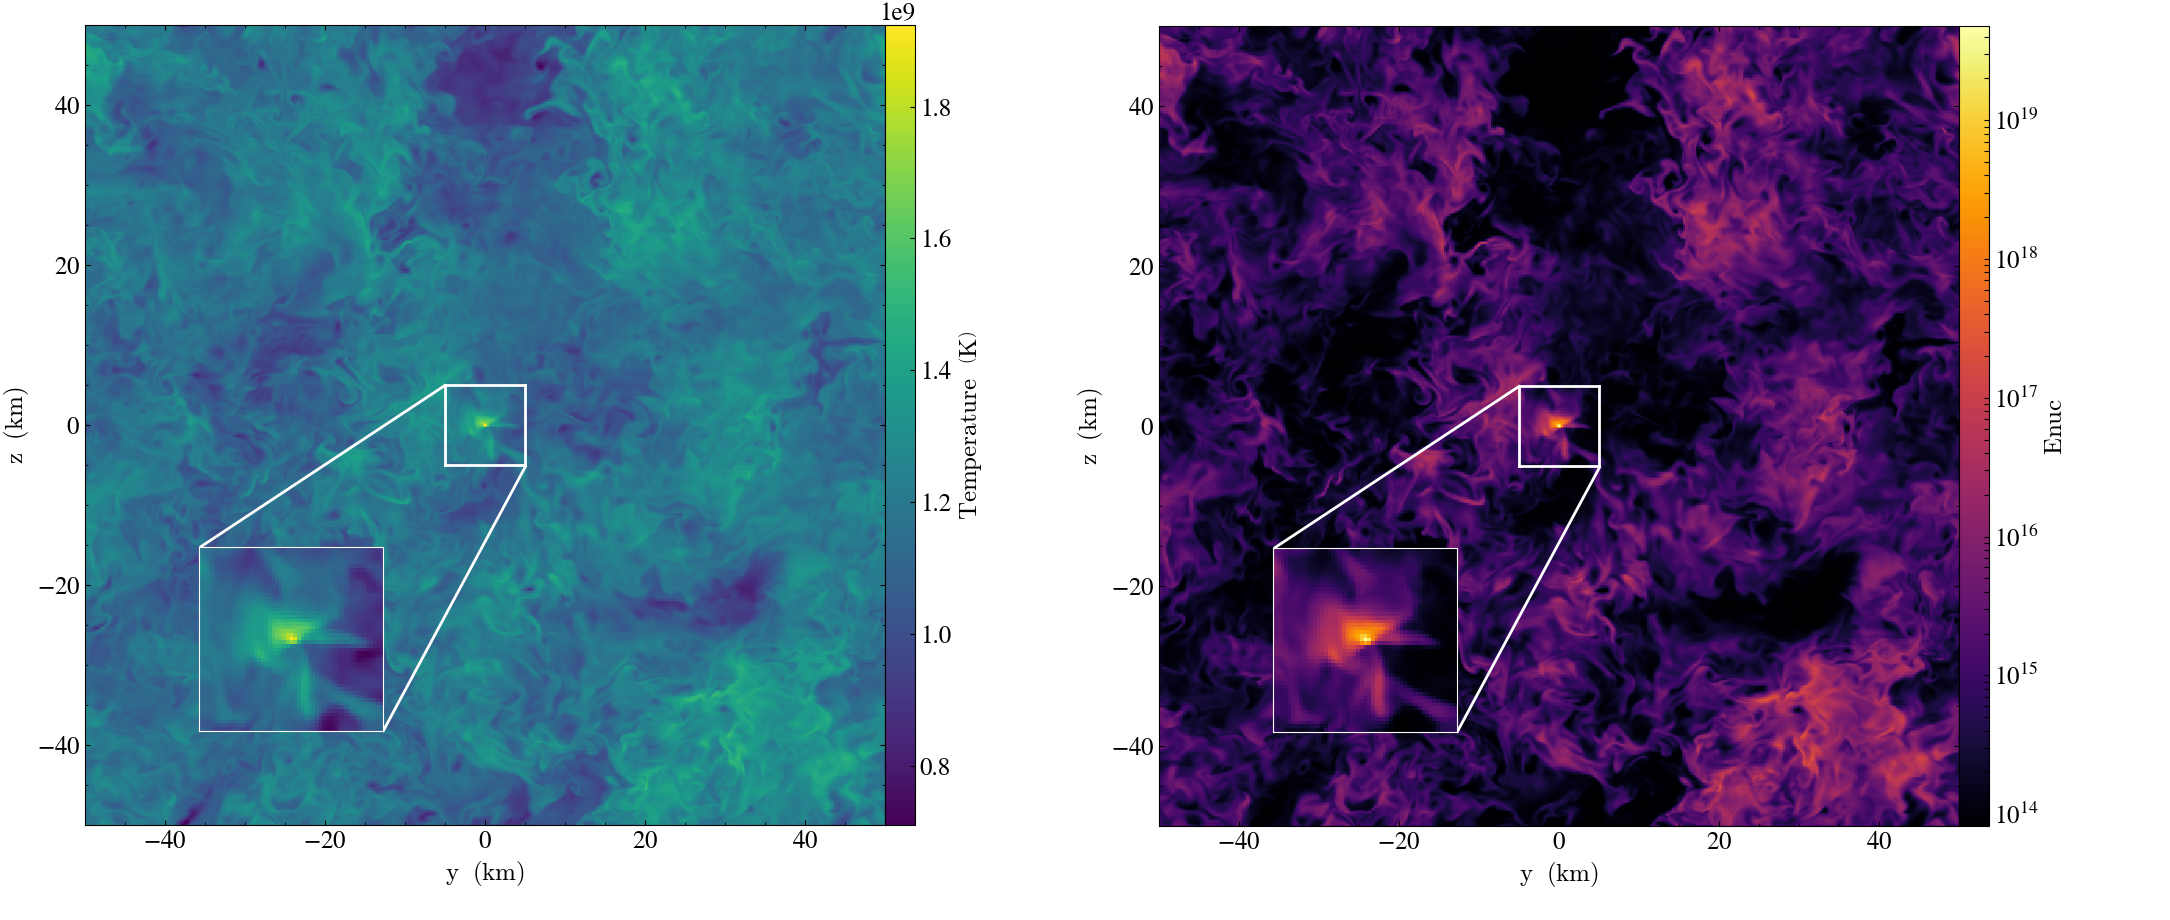
\includegraphics[width=1.0\textwidth]{combined_slice_carbon.png}
\centering
\caption[Slice plots of temperature and specific nuclear energy generation rate, through the maximum temperature in the $z$-$y$ plane, for the $512^3$ run]{Slice plots of temperature and specific nuclear energy generation rate from the C/O run, through the x-axis in the $z$-$y$ plane, for the $512^3$. Each is centered about the hot spot just before leading into a detonation.}
\label {fig:temp_enuc}

\end{figure}
\end{center}

An important implication of these runs is that detonation of carbon can occur in the distributed burning regime through our turbulence mechanism. This is especially important since the Zel'dovich gradient mechanism has been the leading mechanism explaining spontaneous detonation initiation in SNe Ia. Although not wrong, it lacks the physics of turbulence which we know must play a role in the DD channel. From these results, we can now utilize our new mechanism to explore other parameters within these mergers.

\section{Helium Detonation}

Having now a successful detonation mechanism, incorporating helium is a natural next step. As explained before, the detonation of the helium layer of the primary WD opens up the parameter space of how the carbon core can be detonated. Previous work done by Holcomb and collaborators determined tight constraints with regards to temperature, density, and critical length scales for helium burning based upon the Zel'dovich gradient mechanism \cite{holcomb}. They performed one-dimensional hydrodynamic simulations with various initial conditions similar to that which can be modeled with SNe Ia progenitor models. With a turbulently-driven detonation mechanism, we now can perform three-dimensional hydrodynamic simulations and explore the constraints previously modeled.

\section{Simulation Methodology}

Computational tools were used to analyze the physics of turbulence. FLASH, a multiphysics multiscale code built for high-energy density physics, was used to execute three-dimensional hydrodynamic simulations. The hydrodynamics solver used in this case was the split piece-wise parabolic method (PPM). The Helmholtz equation of state was used to incorporate the contributions from nuclei, electrons, blackbody photons, electron-degeneracy, and relativistic effects \cite{timmeswoosley92}. Since this work is only considering a small number of nuclear species, a 19-isotope network was used \cite{weaveretal78}, \cite{timmes99}.

In all, 18 simulations were conducted. Each one had a domain size of $L$ = 100 km, simulated in a fully-periodic box. Spatial resolution ranged from $128^3$ ($L$), $256^3$ ($M$), and $512^3$ ($H$) cells, on a uniform grid. Within each resolution, the parameter space of density and nuclear composition was explored. Densities were set to $10^5$ (LowDen) and $10^6$ (HighDen) g cm$^{-3}$. Initial helium abundance varied from 100\% (PureHe), 25\% (MedHe), and 10\% (MinHe). Carbon and oxygen took up the remaining portion with an assumed equal ratio to one another for each simulation. Initial temperature in all simulations began at $10^8$ K. 

Simulations begin with all the fluid having zero velocity. A large-scale stochastic forcing routine is then used as a stirring mechanism to increase the momentum of the simulation. Each simulation runs until the RMS velocities reach a stable value, indicating that it has reached steady-state turbulence. At this point, the simulations are restarted with nuclear burning turned on and are continued to determine whether detonation will occur. Detonation was classified as the time where helium abundance dropped by 10\% of initial value.

\section{Simulation Results}

Slice plots were generated for temperature and specific nuclear burning using the highest resolution models, $512^3$. A snap shot is taken at the time when the detonation has initiated, with the box centered about the point of maximum temperature, which, owing to the extreme sensitivity of the rates to temperature, is also the point of maximum nuclear burning. At this angle, one is looking through the $x$-axis on the $z$-$y$ plane. Each slice plot has an inset which is zoomed in on the hotspot.

Figure 2.2 shows the slice plots for the MinHeLowDen\_H run, which has a $v_{\rm rms} = 1.26 \times 10^8$ cm s$^{-1}$. For all resolutions, these runs fully detonated helium but saw an increase in carbon abundance, while keeping oxygen almost steady. This implies that the helium was burnt off through the triple-alpha process into carbon. Carbon abundances showed no signs of coming to a detonation.

Figure 2.3 shows the slice plots for the MedHeLowDen\_H run, which has a $v_{\rm rms} = 1.28 \times 10^8$ cm s$^{-1}$. Similar to the previous set of parameters, these runs also saw complete detonation of helium with an increase in carbon, while keeping oxygen steady. This also implies that the triple-alpha process fused most of the helium into carbon, while showing no signs of a carbon detonation.

Figure 2.4 shows the slice plots for the PureHeLowDen\_H run. None of these runs, at all resolutions, detonated. However, helium is seen to also burn into carbon through the triple-alpha process. The slice plots are of the last time step recorded, which has a $v_{\rm rms} = 1.25 \times 10^8$ cm s$^{-1}$. A detonation may be observed if simulations ran long enough but this will explored in more detail in future work.

Figure 2.5 shows the slice plots for the MinHeHighDen\_H run, which has a $v_{\rm rms} = 1.22 \times 10^8$ cm s$^{-1}$. All resolutions of these runs saw a detonation of helium and then of carbon shortly afterwards. They also see a rise in oxygen, which implies that on top of the traditional triple-alpha process occuring, an additional alpha capture on carbon occurs to fuse into oxygen.

Figure 2.6 shows the slice plots for the MedHeHighDen\_H run, which has a $v_{\rm rms} = 5.82 \times 10^7$ cm s$^{-1}$. These runs also show complete detonation of helium and carbon with some formation of oxygen, with indications that heavier elements must have been formed post-detonation.

Figure 2.7 shows the slice plots for the PureHeHighDen\_H run, which has a $v_{\rm rms} = 1.25 \times 10^8$ cm s$^{-1}$. These runs see an almost full detonation of helium, with the abundance ratio falling sharply from 100\% to 20\%. At the onset of detonation, carbon abundance rises from \%0 to near 17.5\%, then immediately fully detonates. Oxygen remains steadily at \%0, indicating again that heavier elements have been formed.

\section{Conclusion}

This body of work confirms that turbulently-driven detonation can occur with various abundance levels of helium, carbon, and oxygen. More specifically, the critical temperature for carbon detonation is robustly a factor of $\sim 2-3$ times lower than theorized from previous studies based upon Zel'dovich. Opening up the parameter space of initial conditions for possible detonation scenarios has been an ongoing endeavour for many decades. With newer observational datasets such as \textit{Gaia}, we can now put constraints on our models and also put our focus on specific channels that match these observations. Further work includes exploring more abundance ratios, higher resolutions, and incorporating more in-depth species networks that would allow us to better understand the nucleosynthesis in these simulations.

\begin{center}
\begin{figure}[!htb]

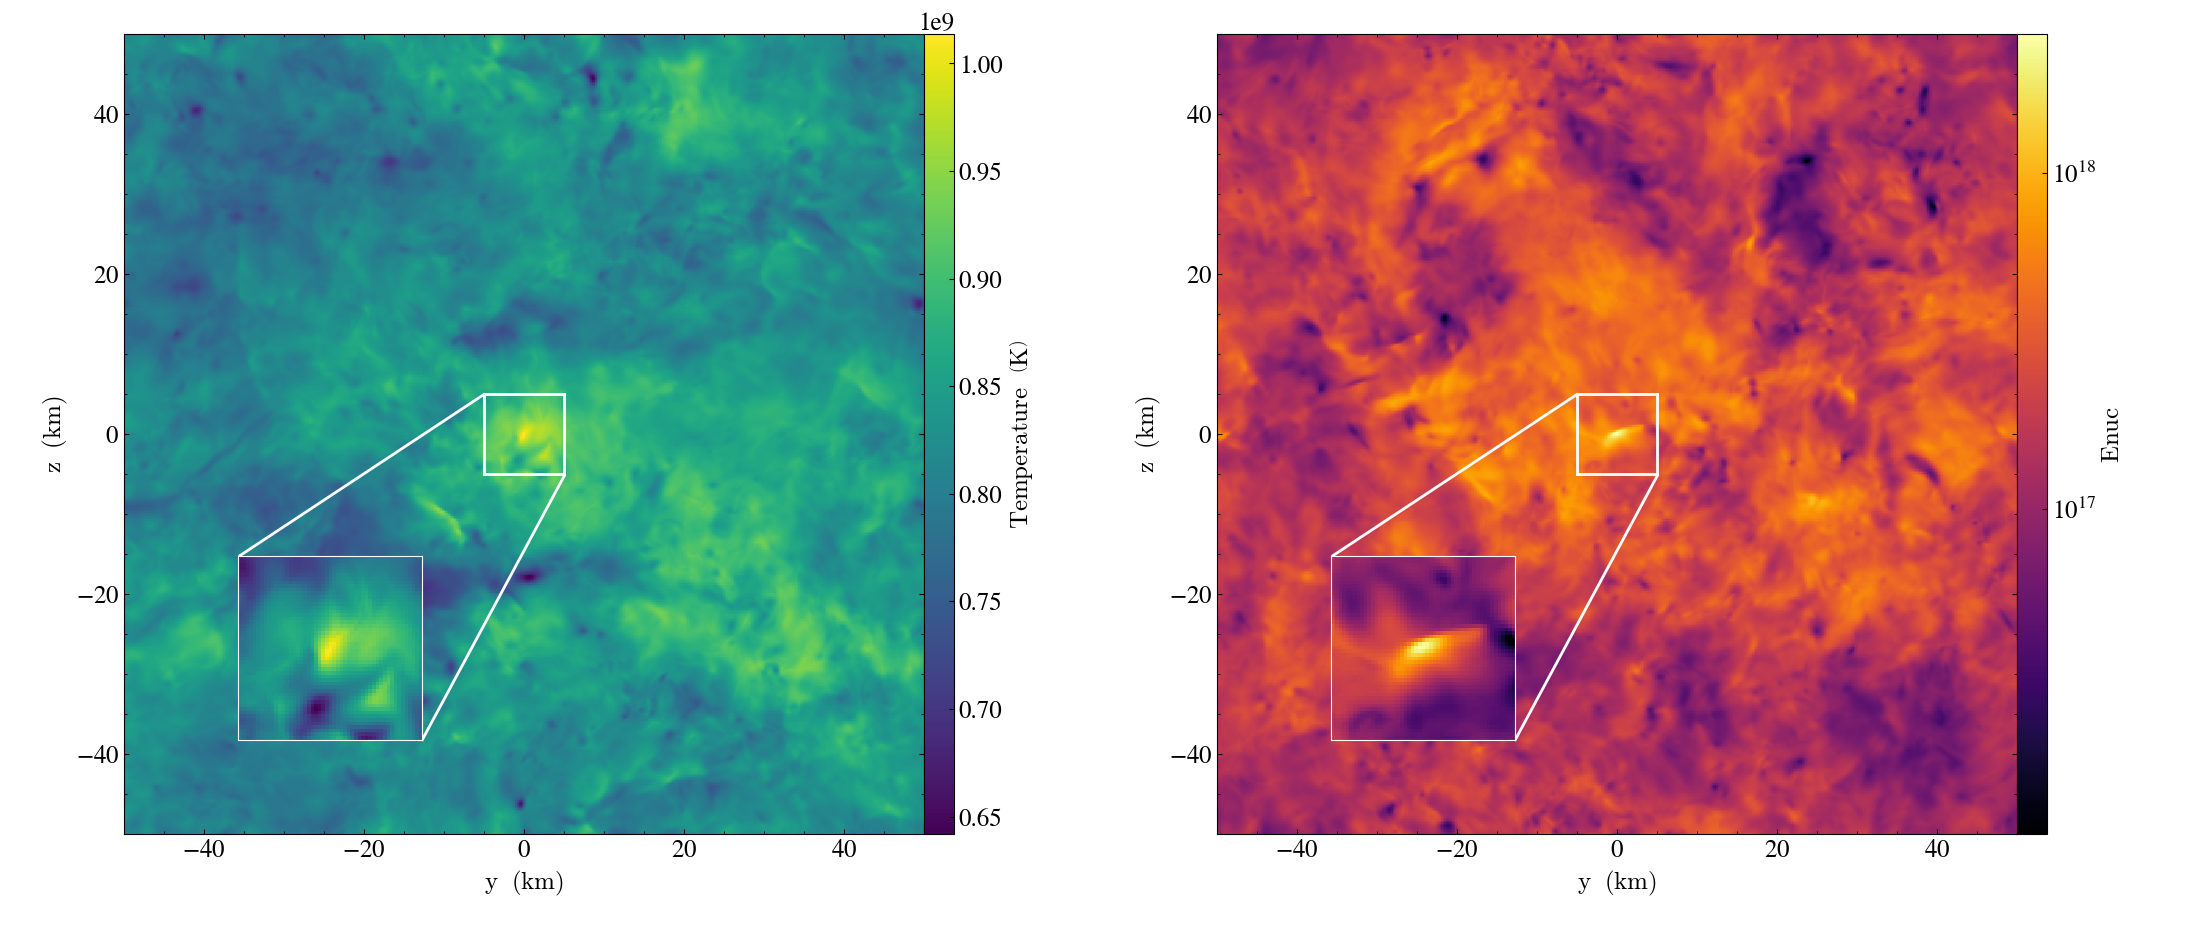
\includegraphics[width=1.0\textwidth]{combined_512_10e5_0.1_new.png}
\centering
\caption[Slice plots of temperature and specific nuclear energy generation rate, for the MinHeLowDen\_H run]{Slice plots of temperature and specific nuclear energy generation rate, for the MinHeLowDen\_H run, through the x-axis in the $z$-$y$ plane, at the onset of detonation.}
\label {fig:temp_enuc}
         
\end{figure}
\end{center}

\begin{center}
\begin{figure}[!htb]

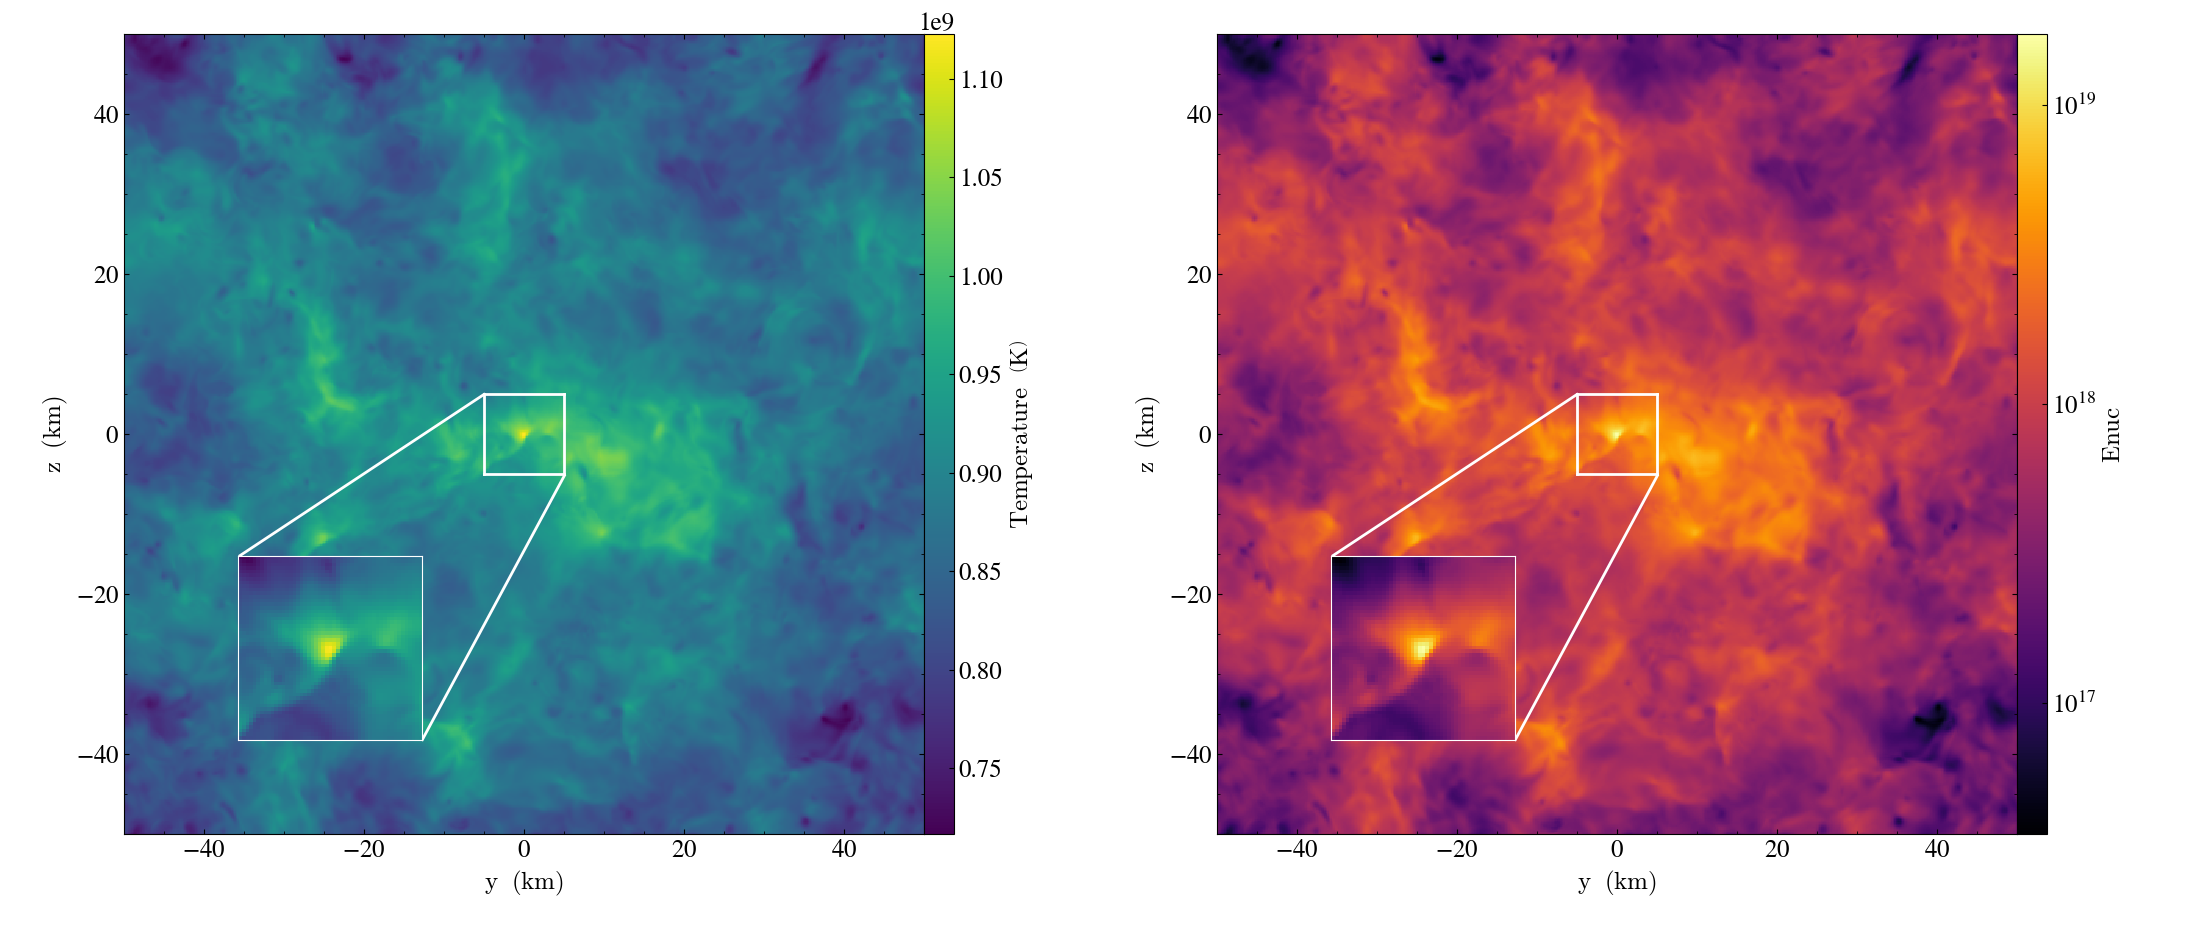
\includegraphics[width=1.0\textwidth]{combined_512_10e5_0.25_new.png}
\centering
\caption[Slice plots of temperature and specific nuclear energy generation rate, for the MedHeLowDen\_H run]{Slice plots of temperature and specific nuclear energy generation rate, for the MedHeLowDen\_H run, through the x-axis in the $z$-$y$ plane, at the onset of detonation.}
\label {fig:temp_enuc}

\end{figure}
\end{center}

\begin{center}
\begin{figure}[!htb]

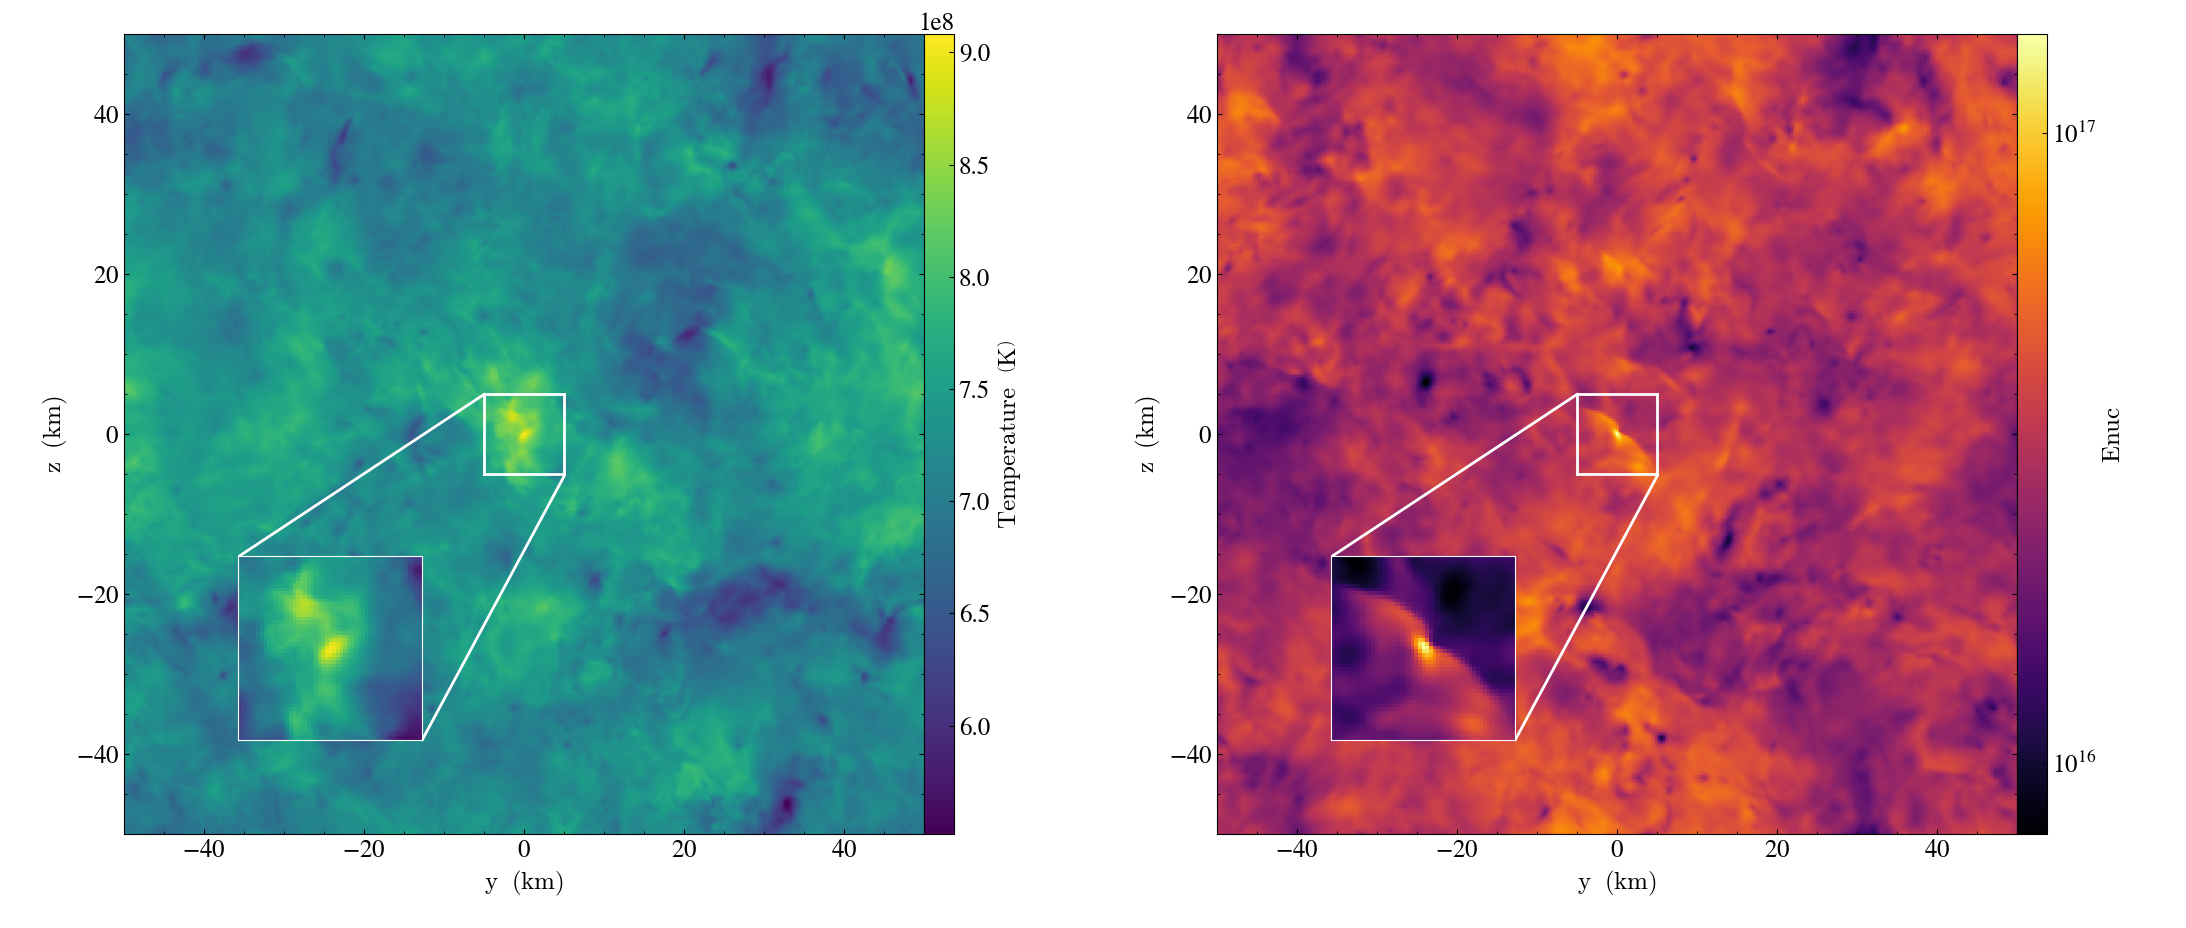
\includegraphics[width=1.0\textwidth]{combined_512_10e5_1.0_new.png}
\centering
\caption[Slice plots of temperature and specific nuclear energy generation rate, for the PureHeLowDen\_H run]{Slice plots of temperature and specific nuclear energy generation ratefor the PureHeLowDen\_H run, through the x-axis in the $z$-$y$ plane, at the last time step of the run.}
\label {fig:temp_enuc}

\end{figure}
\end{center}
\begin{center}
\begin{figure}[!htb]

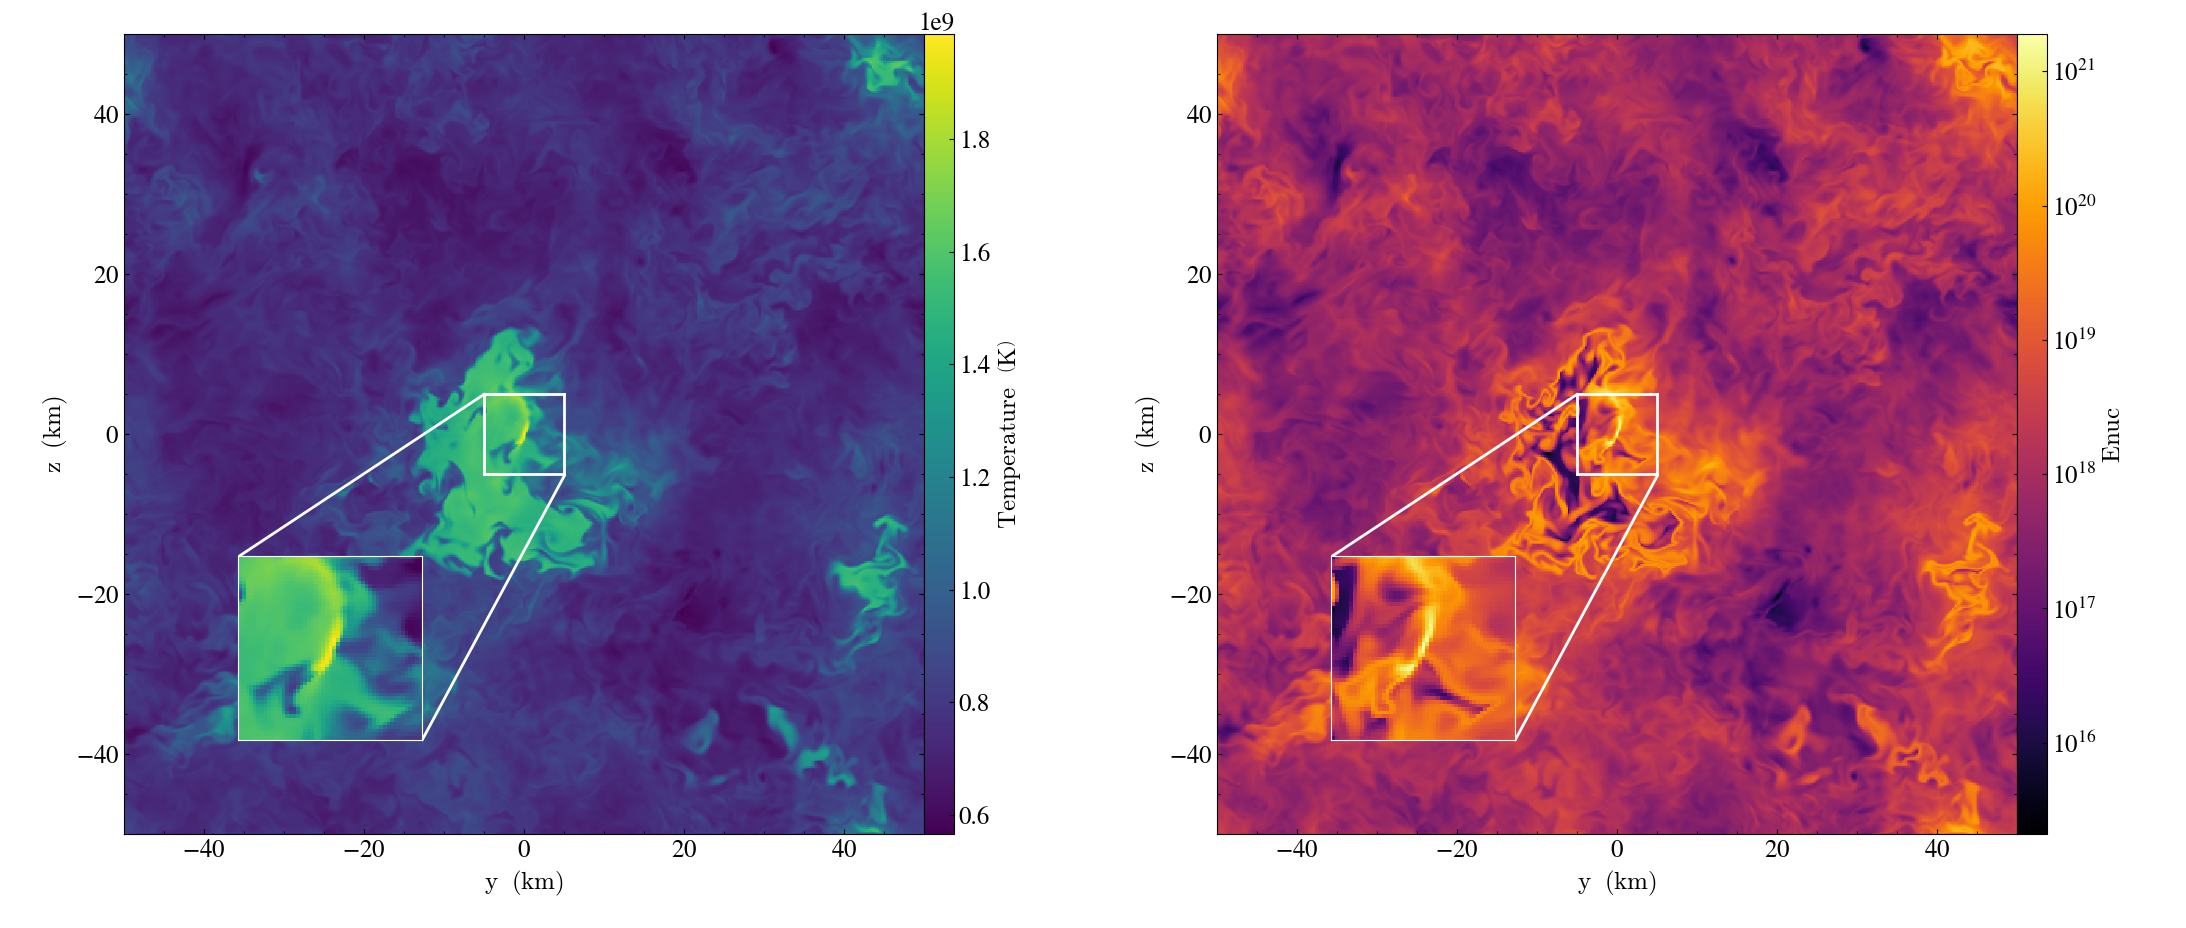
\includegraphics[width=1.0\textwidth]{combined_512_10e6_0.1_new.png}
\centering
\caption[Slice plots of temperature and specific nuclear energy generation rate, for the MinHeHighDen\_H run]{Slice plots of temperature and specific nuclear energy generation rate, for the MinHeHighDen\_H run, through the x-axis in the $z$-$y$ plane, at the onset of detonation.}
\label {fig:temp_enuc}

\end{figure}
\end{center}
\begin{center}
\begin{figure}[!htb]

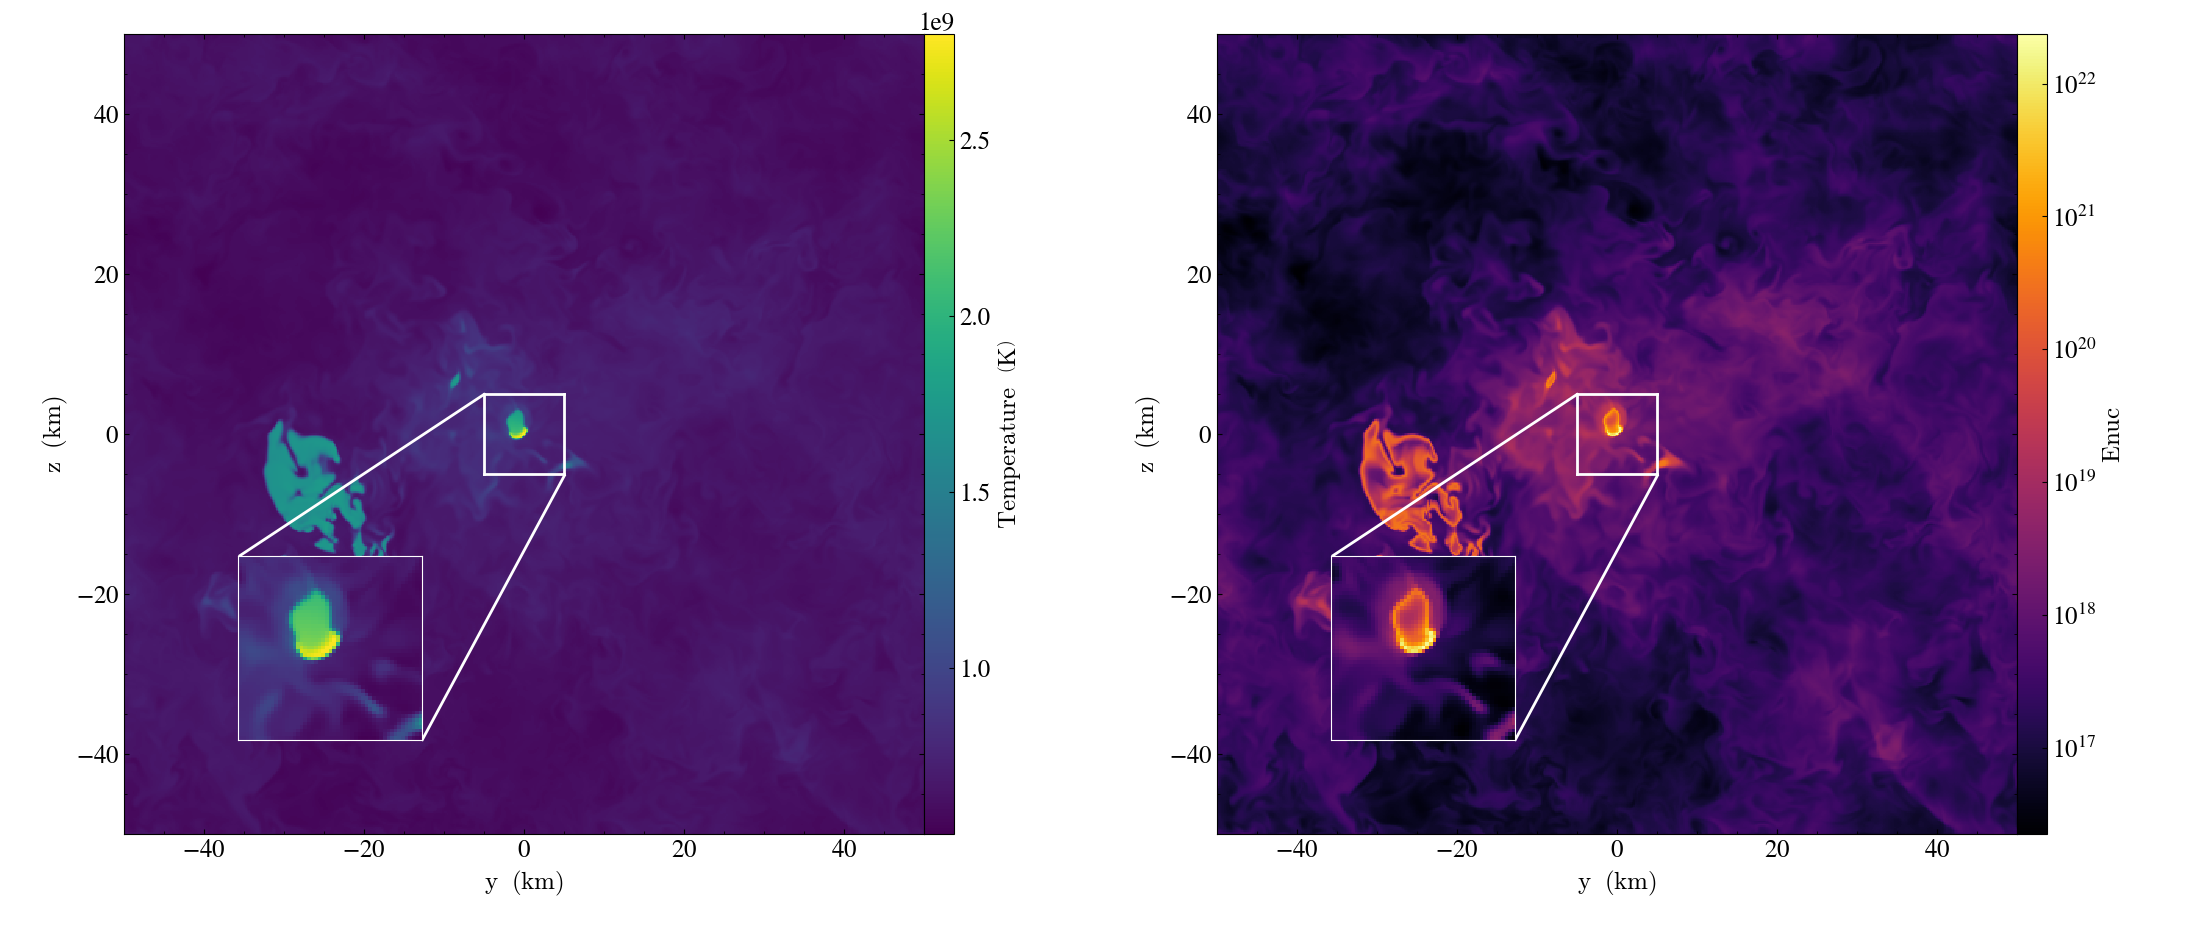
\includegraphics[width=1.0\textwidth]{combined_512_10e6_0.25_new.png}
\centering
\caption[Slice plots of temperature and specific nuclear energy generation rate, for the MedHeHighDen\_H run]{Slice plots of temperature and specific nuclear energy generation rate, for the MedHeHighDen\_H run, through the x-axis in the $z$-$y$ plane, at the onset of detonation.}
\label {fig:temp_enuc}

\end{figure}
\end{center}

\begin{center}
\begin{figure}[!htb]

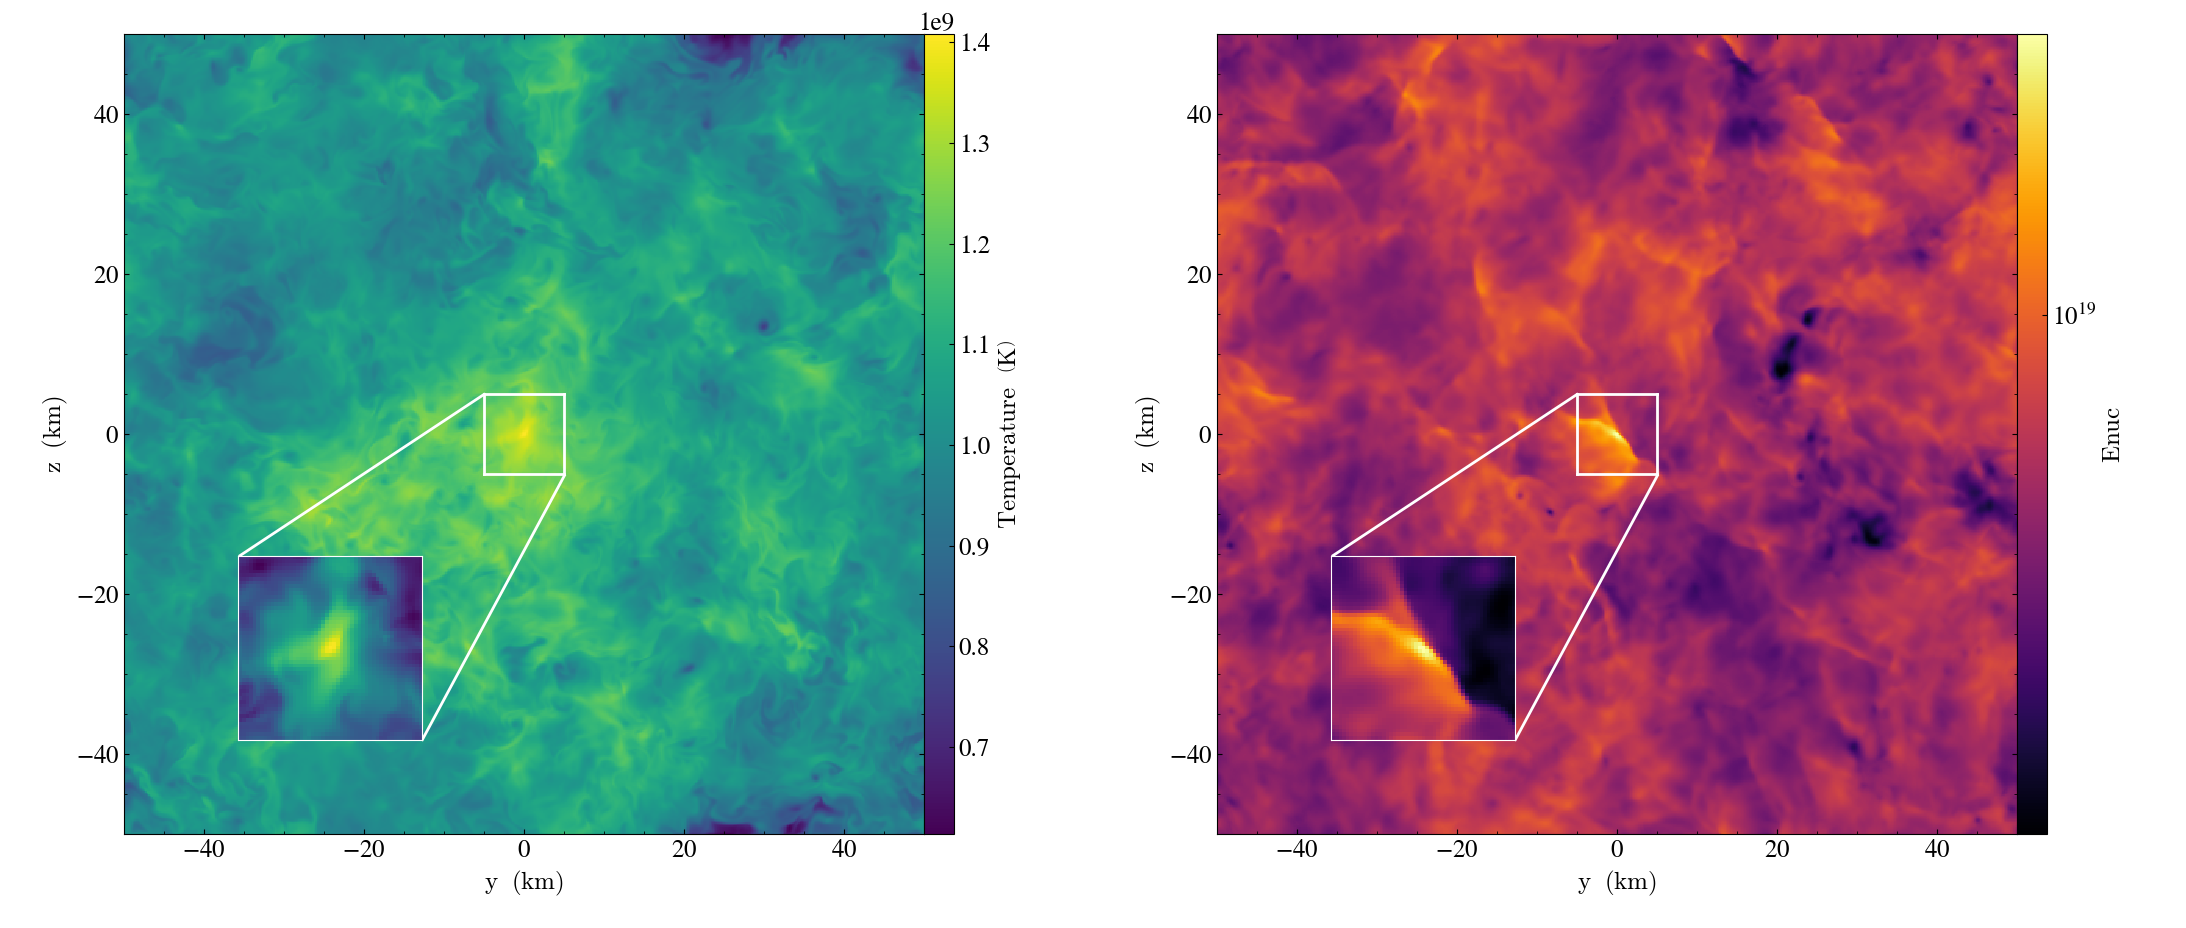
\includegraphics[width=1.0\textwidth]{combined_512_10e6_1.0_new.png}
\centering
\caption[Slice plots of temperature and specific nuclear energy generation rate, for the PureHeHighDen\_H run]{Slice plots of temperature and specific nuclear energy generation rate, for the PureHeHighDen\_H run, through the x-axis in the $z$-$y$ plane, at the onset of detonation.}
\label {fig:temp_enuc}

\end{figure}
\end{center}

\begin{table}[!htb]
        \caption[A table of helium-carbon-oxygen runs with different resolution, RMS velocity and mean temperature..]{A table of runs with the different resolutions, densities, helium abundances, and mean temperature at the time of detonation initiation, $T_{\rm det}$ (K).}
  \begin{center}
      \begin{tabular}{|c|c|c|c|}
        \hline
              Resolution & Density (g cm$^{-3}$) & Helium Abundance & $T_{\rm det}$ (K)\\
        \hline\hline
        $128^3$   & $10^5$ & 0.1 & $8.22 \times 10^8$  \\
        $128^3$   & $10^5$ & 0.25 & $8.77 \times 10^8$  \\
        $128^3$   & $10^5$ & 1.0 & None  \\
        $128^3$   & $10^6$ & 0.1 & $7.80 \times 10^8$  \\
        $128^3$   & $10^6$ & 0.25 & $7.87 \times 10^8$  \\
        $128^3$   & $10^6$ & 1.0 & $9.91 \times 10^8$  \\
        $256^3$   & $10^5$ & 0.1 & $8.25 \times 10^8$  \\
        $256^3$   & $10^5$ & 0.25 & $8.83 \times 10^8$  \\
        $256^3$   & $10^5$ & 1.0 & None  \\
        $256^3$   & $10^6$ & 0.1 & $7.99 \times 10^8$  \\
        $256^3$   & $10^6$ & 0.25 & $8.81 \times 10^8$  \\
        $256^3$   & $10^6$ & 1.0 & $1.09 \times 10^9$  \\
        $512^3$   & $10^5$ & 0.1 & $8.28 \times 10^8$  \\
        $512^3$   & $10^5$ & 0.25 & $8.75 \times 10^8$  \\
        $512^3$   & $10^5$ & 1.0 & None  \\
        $512^3$   & $10^6$ & 0.1 & $7.80 \times 10^8$  \\
        $512^3$   & $10^6$ & 0.25 & $6.30 \times 10^8$  \\
        $512^3$   & $10^6$ & 1.0 & $1.06 \times 10^9$  \\
        \hline
   \end{tabular}
  \end{center}
  \label{runs}
\end{table}


%\chapter{Tests}

\section{Spatial-Resolution Convergence}


%\section{Kolmogorov's Theory}


\section{Analytic Curves}



%%\input{conclusion}

%\singleappendix
%\input{appendix}



%%%
%%%  If there is ONE appendix use the \singleappendix command
%%%
%\singleappendix
%\chapter{The Only Appendix}
%
%If there is only one appendix, it is called ``Appendix'' (not ``Appendix
%A'').  
%
%To achieve this, use the command, {\tt $\backslash$singleappendix}
%
%\section{Appendictical Numbering}
%\label{sample-appendix:numbering-section}
%
%The command, {\tt $\backslash$singleappendix} prints the appendix title without
%the trailing A.
%
%\section{Getting the labels right \ldots}
%
%The {\tt $\backslash$singleappendix} command also ensures that the section and
%subsection numbers don't include a leading A. and  that the the Table of
%Contents, List of Figures and List of Tables entries for section, subsection,
%equations, figures and tables don't have a leading period. 
%
%\begin{equation}
%  a_{i} = b^{2x} + c\times\gamma - \frac{1}{5} \sin\theta
%\end{equation}
%
%\begin{figure}[htbp]
%% the optional arguments htbp tell LaTeX where on the page the figure 
%% should be placed. In order this argument means try putting it "here", 
%% at the "top", at the "bottom" or (as a last resort) on a seperate "page"
%\begin{center}
%  \includegraphics[width=0.40\textwidth,keepaspectratio]{sample_fig.png}
%  \caption{
%    \label{sample2-figure}% so we can cross-reference the figure
%    This is a small figure.}%
%  \end{center}
%\end{figure}

%%
%%  End of any appendices
%%  =========================================================================


%%  At the end of the document are the references. These are single-spaced
%%  rather than double-spaced like the rest of the thesis text.

\begin{doublespace}
     \begin{thebibliography}{11}

%\iffalse
\bibitem{holcomb} C. Holcomb {\it et al}, Astrophysical Journal {\bf 771}, 14 (2013).


\bibitem{euler} J.K. Truelove {\it et al}, Astrophysical Journal {\bf 495}, 821 (1998).


\bibitem{Gaia} K. Shen {\it et al}, Astrophysical Journal {\bf 865}, 14 (2018).

\bibitem{Shen} K. Shen {\it et al}, Astrophysical Journal {\bf 854}, 15 (2018).

\bibitem{giammichele} N. Giammichele {\it et al.}, Nature {\bf 554}, 73 (2018).

\bibitem{Fisher} R. Fisher {\it et al.}, Astrophysical Journal {\bf 876}, 64 (2019).
	
%\bibitem{Clayton} D. D. Clayton, {\it Principles of Stellar Evolution and Nucleosynthesis}, University of Chicago Press, 1968.

\bibitem{Nugent_2011} P. E. Nugent {\it et al.}, Nature {\bf480},  344 (2011).

\bibitem{phillips93} M. M. Phillips, Astrophysical Journal Letters {\bf 413}, L105 (1993).

\bibitem{Riess98} Riess {\it et al.}, Astrophysical Journal {\bf 116}, 1009 (1998).

%\bibitem{Whelan&Iben1973} J. Whelan and I. I. JR., Astrophysical Journal {\bf 186}, 1007 (1973).

%\bibitem{Arnett1969} W. D. Arnett and  J. W. Truran, Astrophysical Journal {\bf 157}, 339 (1969).

%\bibitem{Khokhlov1991} A. M. Khokhlov, Astronomy and Astrophysics {\bf 245}, 114 (1991).

%\bibitem{baadezwicky34} W. Baade and F. Zwicky, Proceedings of the National Academy of Science {\bf 20}, 259 (1934).

%\bibitem{ginzburg64} V. L. Ginzburg and S. I. Syrovatskii, {\it The Origin of Cosmic Rays}, New York: Macmillan, 1964.

%\bibitem{drury12} L. O. Drury, Astroparticle Physics {\bf 39}, 52 (2012), arXiv: 1203.3681.

%\bibitem{elmegreenscalo04} B. G. Elmegreen and J. Scalo, Annual Review of Astronomy and Astrophysics {\bf 42}, 211 (2004), astro-ph/0404451.

%\bibitem{kobayashietal06} C. Kobayashi {\it et al.}, Astrophysical Journal {\bf 653}, 1145 (2006), astro-ph/0608688.

%\bibitem{blinnikovkhoklhlov86} S. I. Blinnikov and A. M. Khokhlov, Soviet Astronomy Letters {\bf 12}, 131 (1986).

%\bibitem{blinnikovkhoklov87} S. I. Blinnikov and A. M. Khokhlov, Soviet Astronomy Letters {\bf 13}, 364 (1987).

\bibitem{zeldovichetal70} Y. B. Zel’dovich {\it et al.}, Journal of Applied Mechanics and Technical Physics {\bf 11}, 264 (1970).

%\bibitem{guillochonetal10} J. Guillochon {\it et al.}, Astrophysical Journal Letters {\bf 709}, L64 (2010), arXiv:0911.0416.

%\bibitem{pakmor_etal_2013} R. Pakmor {\it et al.}, Astrophysical Journal Letters {\bf 770}, L8 (2013), arXiv:1302.2913.

%\bibitem{khokhlovetal97} A. M. Khokhlov {\it et al.}, Astrophys. J. {\bf 478}, 678 (1997), arXiv:astro-ph/9612226.

%\bibitem{arnettlivne94} D. Arnett and E. Livne, Astrophys. J. {\bf 427}, 330 (1994).

%\bibitem{niemeyerwoosley97} J. C. Niemeyer and S. E. Woosley, Astrophys. J. {\bf 475}, 740 (1997), arXiv:astro-ph/9607032.

%\bibitem{ropkeetal07a} F. K. Röpke {\it et al.}, Astrophys. J. {\bf 660}, 1344 (2007), astro-ph/0609088.

%\bibitem{seitenzahletal09a} I. R. Seitenzahl {\it et al.}, Astrophys. J. {\bf 696}, 515 (2009), arXiv:0901.3677.

%\bibitem{holcombetal13} C. Holcomb {\it et al.}, Astrophys. J. {\bf 771}, 14 (2013), arXiv:1302.6235.

%\bibitem{nandkumarpethick84} R. Nandkumar and C. J. Pethick, Monthly Notices of the Royal Astronomical Society {\bf 209}, 511 (1984).

%\bibitem{garciasenzwoosley95} D. Garcia-Senz and S. E. Woosley, Astrophys. J. {\bf 454}, 895 (1995).

%\bibitem{danetal14}M. Dan {\it et al.}, Monthly Notices of the Royal Astronomical Society {\bf 438}, 14 (2014), arXiv:1308.1667.

%\bibitem{aspdenetal08}A. J. Aspden {\it et al.}, Astrophys. J. {\bf 689}, 1173-1185 (2008), arXiv:0811.2816.

%\bibitem{woosley07}S. E. Woosley, Astrophys. J. {\bf 668}, 1109 (2007), arXiv:0709.4237.

\bibitem{timmeswoosley92} F. X. Timmes and S. E. Woosley, Astrophys. J. {\bf 396}, 649 (1992).

%\bibitem{woosley97} S. E. Woosley, Astrophys. J. {\bf 476}, 801 (1997).

%\bibitem{sheleveque94} Z. S. She and E. Leveque, Phys. Rev. Lett. {\bf 72}, 336 (1994).

%\bibitem{dubrelle94} B. Dubrulle, Phys. Rev. Lett. {\bf 73}, 959 (1994).

%\bibitem{fennplewa17} D. Fenn and T. Plewa, Monthly Notices of the Royal Astronomical Society {\bf 468}, 1361 (2017), arXiv:1703.00432.

%\bibitem{Timmes_2000} F. X. Timmes and F. D. Swesty, The Astrophysical Journal Supplement Series {\bf 126}, 501–516 (2000).

\bibitem{weaveretal78} T. A. Weaver {\it et al.}, Astrophys. J. 225, 1021 (1978).

\bibitem{timmes99} F. X. Timmes, Astrophysical Journal Supplement {\bf 124}, 241 (1999).

%\bibitem{benzietal08} R. Benzi {\it et al.}, Physical Review Letters {\bf 100}, 234503 (2008), arXiv:0709.3073.

%\bibitem{arneodoetal08} A. Arnèodo {\it et al.}, Physical Review Letters {\bf 100}, 254504 (2008).

%\bibitem{benzietal10} R. Benzi {\it et al.}, Journal of Fluid Mechanics {\bf 653}, 221 (2010).

%\bibitem{federrathetal10} C. Federrath {\it et al.}, Astronomy \& Astrophysics {\bf 512}, A81 (2010), arXiv:0905.1060.

%\bibitem{Hawley_etal_2012} W. P. Hawley, T. Athanassiadou, and F. X. Timmes, Astrophys. J. {\bf 759}, 39 (2012), arXiv:1209.3749.

%\bibitem{kashyapetal15} R. Kashyap {\it et al.}, Astrophysical Journal Letters {\bf 800}, L7 (2015), arXiv:1501.05645.

%\bibitem{pakmoretal10} R. Pakmor {\it et al.}, Nature (London) {\bf 463}, 61 (2010), arXiv:0911.0926.

%\bibitem{molletal14} R. Moll {\it et al.},  Astrophys. J. {\bf 785}, 105 (2014), arXiv:1311.5008.

%\bibitem{bullaetal16} M. Bulla {\it et al.}, Monthly Notices of the Royal Astronomical Society {\bf 455}, 1060 (2016), arXiv:1510.04128 [astro-ph.HE].

%\bibitem{kushniretal13} D. Kushnir {\it et al.}, Astrophysical Journal Letters {\bf 778}, L37 (2013), arXiv:1303.1180 [astro-ph.HE].

%\bibitem {Turk_2011} M. J. Turk {\it et al.}, The Astrophysical Journal Supplement Series {\bf 192}, 9 (2011).

%\bibitem{Benzietal93} R. Benzi {\it et al.}, Physical Review E {\bf48}, R29 (1993).   

%\fi
\end{thebibliography}
 
 
 

 

\end{doublespace} 
     
%\end{singlespace}
   
\end{document}
%% ===========
%%    FINI
%% ===========
